% !TEX encoding = UTF-8
% !TEX TS-program = pdflatex
% !TEX root = ../tesi.tex

%**************************************************************
\chapter{Testing}
\label{cap:test}
%**************************************************************
\intro{Nel seguente capitolo verranno descritte le tecnologie utilizzate per costruire una test-suite per l'applicazione mobile e verrà esposto il piano di \emph{test} stabilito con il tutor aziendale inserendo i risultati ottenuti.}
\section{Test End to End}
Il \emph{test End-to-End} è una metodologia di \emph{testing} dell'interfaccia grafica che viene vista dagli utenti dell'applicazione. Ha lo scopo di testare in modo automatizzato se, tutti flussi di esecuzione dell'applicazione, dall'inizio fino alla fine, si stanno comportando come progettato, senza che vengano rilevati degli errori che andrebbero a inficiare sulla qualità dell’applicazione stessa. Perciò il \emph{test} \gls{test e2e} consiste nel simulare degli scenari utente reali ad esempio interazioni attraverso clic sui bottoni da parte degli utenti, in modo da verificare che l'applicazione si comporti nel modo corretto garantendo che vengano soddisfati i requisiti di alto livello del prodotto. Quindi il \emph{test} \gls{test e2e} verifica l'intera applicazione su tutte le possibili interazione che l'utente può fare, testando inoltre, se vengono trasmesse le informazioni corrette tra le varie componenti dell'applicazione garantendo che l'applicazione funzioni come un unico sistema coerente. Un esempio di \emph{test} \gls{test e2e} possono essere la simulazione dei passi che l'utente deve fare per autenticarsi nell'applicazione, quindi il \emph{test} può essere così composto:
\begin{enumerate}
	\item Inserisci l'\emph{username} nella casella di testo;
	\item Inserisci la \emph{password} nella casella di testo;
	\item Clicca il bottone di \emph{login};
	\item Verifica che ti trovi nella pagina principale dell'applicazione dopo l'autenticazione e non più nella pagina di \emph{login}.
\end{enumerate}

Come scritto, i \emph{test} \gls{test e2e} eseguono l'applicazione proprio come se fosse un utente in un ambiente il più vicino possibile alla realtà. Proprio come un utente, i \emph{test} \gls{test e2e} dovrebbero avere una comprensione praticamente nulla dei componenti interni dell'applicazione perché si vuole evitare accoppiamenti non necessari. Infatti, i test di unità e di integrazione sono i luoghi in cui dovrebbe essere nota la composizione interna dell'applicazione, e quindi dove i mock possono essere utilizzati per attivare particolari rami di codice che si ha l'esigenza di testare. Il fatto che i \emph{test} \gls{test e2e} non sanno la struttura interna e il funzionamento dell'applicazione che stanno testando li classifica come \emph{test} \emph{black-box}.
\clearpage

\begin{figure}[!h] 
	\begin{center}
		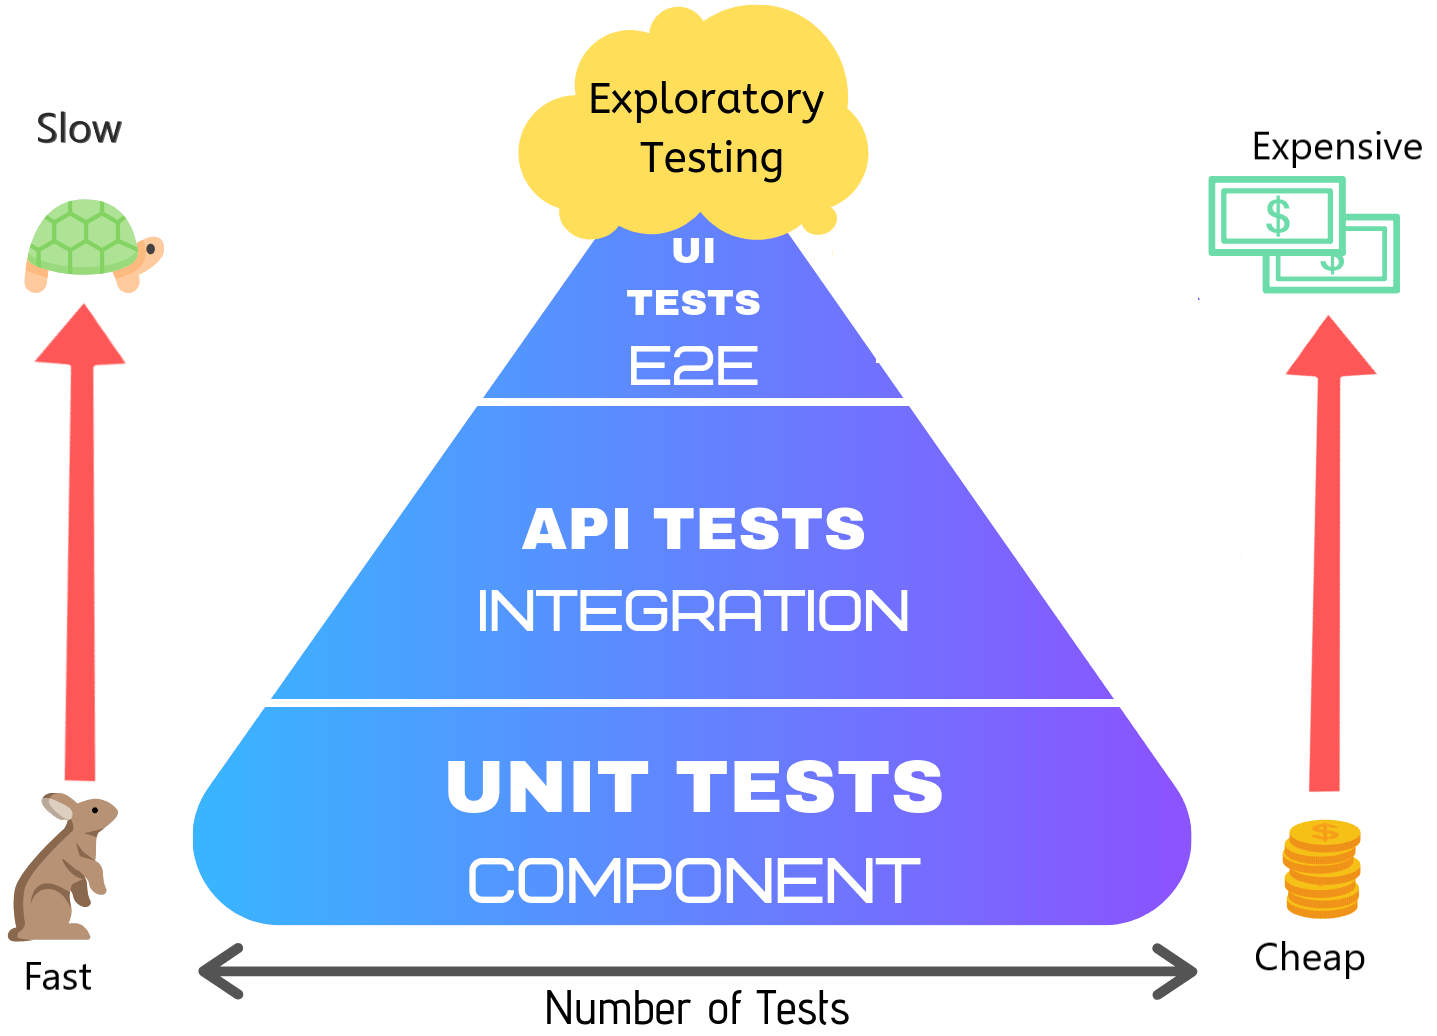
\includegraphics[scale=0.3]{piramideTest.png}
		\caption{Piramide dei test}\label{fig:test}
	\end{center}
\end{figure}

Come mostra la Figura~\ref{fig:test}, la piramide dei \emph{test} illustra il numero proporzionale di \emph{test} per ogni tipologia di \emph{test} in relazione alla loro velocità d'esecuzione e costi per implementarli. Sebbene i \emph{test} \gls{test e2e} forniscano un grande supporto per testare la correttezza dell'applicazione, sono significativamente più lenti e più costosi rispetto ai test unitari, a causa della loro elevata complessità e onerosità computazionale. Perciò è fondamentale trovare il giusto equilibrio di \emph{test} \gls{test e2e} da implementare senza perderne i vantaggi e senza aumentare i costi per l'implementazione. Una buona applicazione di \emph{test} \gls{test e2e} può essere ad esempio il \emph{testing} di azioni ripetitive che grazie alla fatto che sono \emph{test} automatizzati, risultano essere meno costosi è più efficaci rispetto ai \emph{test} manuali.

\section{Tecnologie per il testing}
Per implementare i \emph{test} \gls{test e2e} sia per la \emph{dashboard} di \gls{AWMS} sia per l'applicazione \emph{mobile} si sono usare diverse tecnologie tra loro. Per il \emph{testing} della \emph{dashboard} si sono usate le seguenti tecnologie:
\begin{itemize}
	\item \textbf{Selenium WebDrive};
	\item \textbf{Protractor};
	\item \textbf{Cucumber}.
\end{itemize}
Selenium è un \gls{framework}\ap{[g]} che permette di automatizzare l'esecuzione dei \emph{test} all'interno dei \gls{browser web}\ap{[g]}. Ciò è possibile grazie a un insieme di \gls{api}\ap{[g]} detto API WebDriver. Queste \gls{api}\ap{[g]} sono uno standard W3C che rappresentano un'interfaccia di controllo remoto che consente di manipolare elementi del DOM nelle pagine web e di comandare il comportamento dei programmi utente. Inoltre, fornisce un protocollo, noto come JSON Wire Protocol, per il trasferimento dei dati per varie piattaforme che permettono di automatizzare i \emph{test} sui \gls{browser web}\ap{[g]} come:
\begin{itemize}
	\item GeckoDriver per Mozilla Firefox;
	\item ChromeDriver per Google Chrome;
	\item SafariDriver per Apple Safari;
	\item InternetExplorerDriver per Microsoft Internet Explorer;
	\item MicrosoftWebDriver o EdgeDriver per Microsoft Edge;
	\item OperaChromiumDriver per Opera.
\end{itemize}
Selenium per eseguire i \emph{test} utilizza un’architettura client-server infatti, Selenium utilizza un server web dove espone l'API WebDriver come API REST. Perciò rimane in ascolto per la ricezione dei comandi che compongono i \emph{test}, sotto forma di richieste HTTP. Quando arrivano le richieste le esegue su un \gls{browser web}\ap{[g]} e risponde con una risposta HTTP che rappresenta il risultato dell'esecuzione del comando. Grazie alla standardizzazione delle \gls{api}\ap{[g]} e l'utilizzo di un architettura client-server è possibile eseguire \emph{test} scritti in diversi linguaggi purché supportino l'invio di richieste HTTP.

Protractor è un \gls{framework}\ap{[g]} di \emph{test} \gls{test e2e} per applicazioni Angular2+ e AngularJS. Protractor offre un insieme di "localizzatori" cioè metodi che permettono di ricavare gli elementi o il valore degli attributi dall'applicazione web, ma anche di simulare dei \emph{click} come se fosse un utente umano. Per funzionare Protractor all'inizio richiede che sia presente un server Selenium in modo da mandare richieste HTTP per eseguire i \emph{test} \gls{test e2e}.

\begin{figure}[h] 
	\begin{center}
		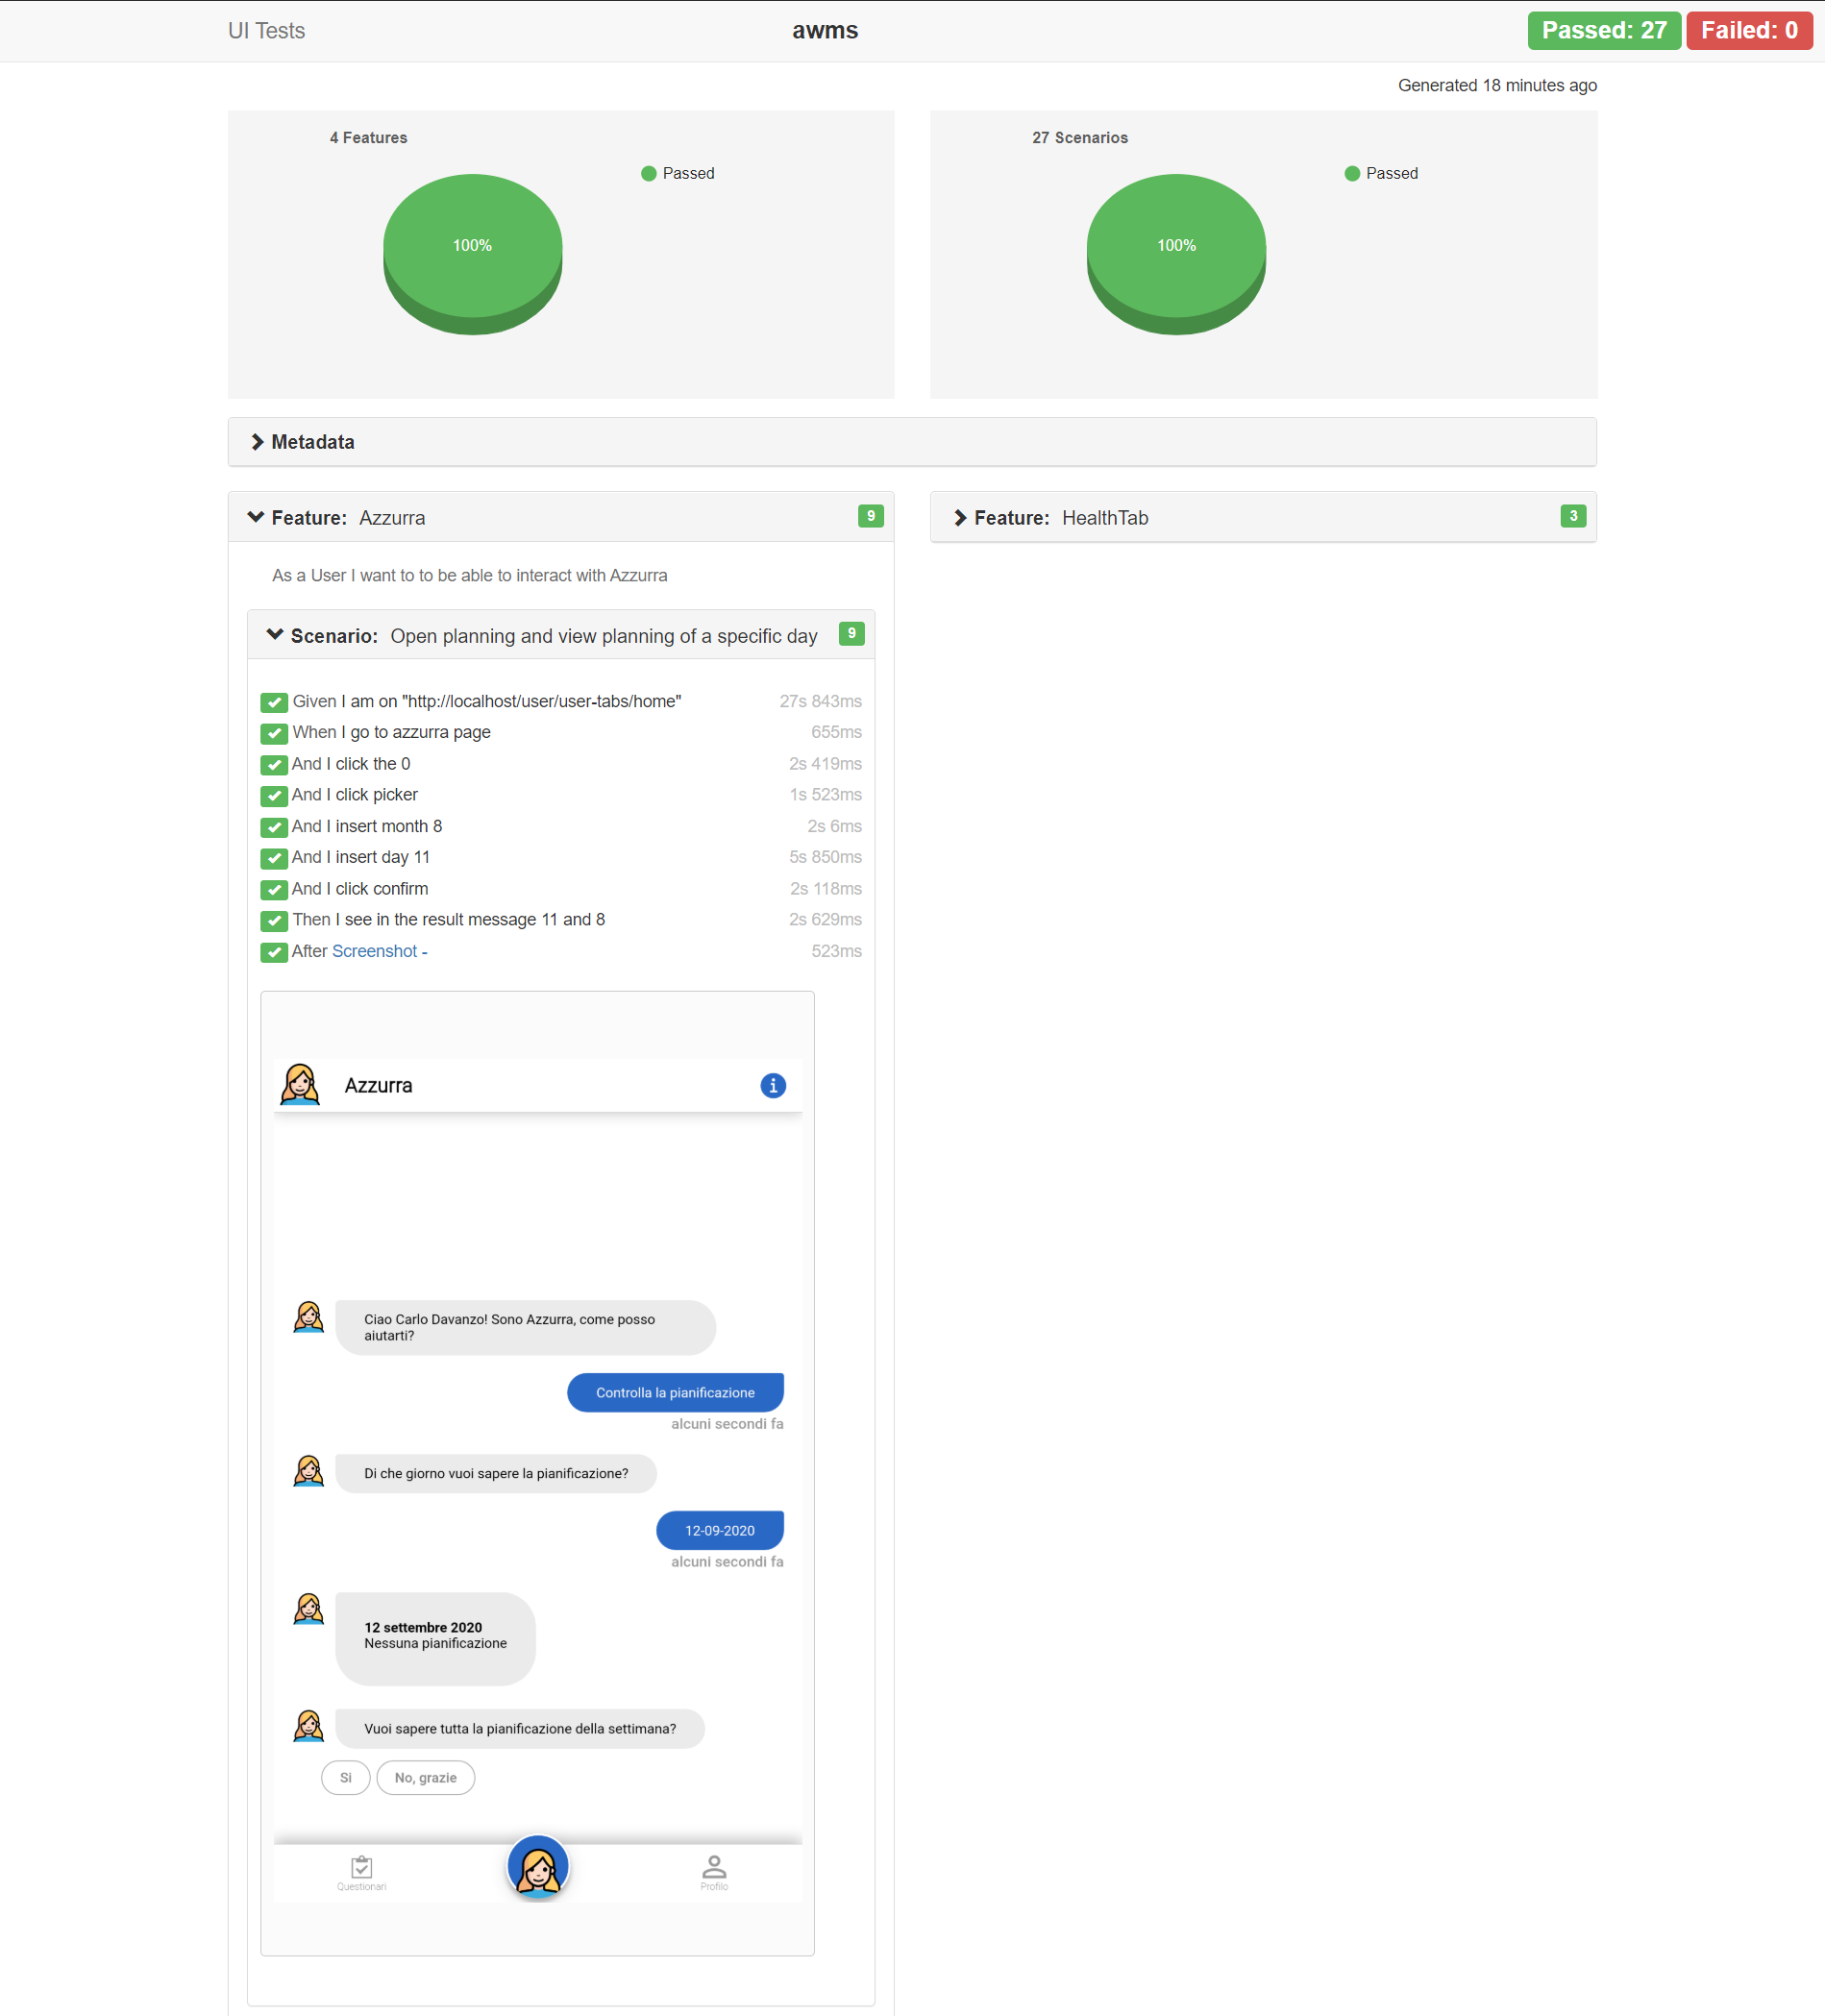
\includegraphics[height=20cm, width=13cm]{report.png}
		\caption{Una parte del report dei test per il mobile generato da Cucumber}\label{fig:testDoc}
	\end{center}
\end{figure}

Infine, Cucumber permette di definire i vari passi che deve fare un \emph{test} automatizzato per simulare le azioni di un utente. Questi passi vengono dichiarati attraverso il linguaggio Gherkin, un linguaggio di facile comprensione. Quindi grazie a Cucumber vengono dichiarati i cosiddetti \emph{step} cioè i passi che devono essere fatti all'interno del \emph{test}, l'insieme dei \emph{step} definisce lo scenario dei test, ad esempio uno scenario di test può essere il processo di autenticazioni e gli \emph{step} sono l'inserimento dei dati e l'invio. I vari \emph{step} vengono poi implementati in un linguaggio di programmazione, in questo caso TypeScript utilizzando i metodi offerti da Protractor. Il fatto che vengano dichiarati i passi che il \emph{test} permettono a Cucumber di supportare la BDD. Quando vengono eseguiti i \emph{test} Cucumber controlla se Selenium sta eseguendo le azioni specificate all’interno di un \gls{browser web}\ap{[g]}. Al termine dell'esecuzione Cucumber riesce a stabilire l'esito per ogni \emph{test} inoltre, produce dei \emph{report} sui \emph{test} appena eseguiti documentandone l'esito e la struttura come mostrato in Figura~\ref{fig:testDoc}.
\clearpage
Per l'applicazione \emph{mobile} si è continuato a utilizzare Protractor e Cucumber ma al posto di Selenium si è utilizzato Appium. Viene utilizzato Appium perché offre l'automazione dei \emph{test} per applicazioni native, web mobile e ibride, con la particolarità di essere multi-piattaforma cioè può eseguire i \emph{test} sia su \gls{iOS}\ap{[g]} e \gls{Android}\ap{[g]}. Selenium invece non permette l'esecuzione di \emph{test} su dispositivi \emph{mobile} ma solo su \gls{browser web}\ap{[g]}. Appium utilizza la stessa architettura client-server di Selenium inoltre da esso ne prende anche l'utilizzo dell'API WebDriver in particolare viene utilizzato una variante per il \emph{mobile} del protocollo JSON Wire Protocol noto con il nome di Mobile JSON Wire Protocol. 

\begin{figure}[h] 
	\begin{center}
		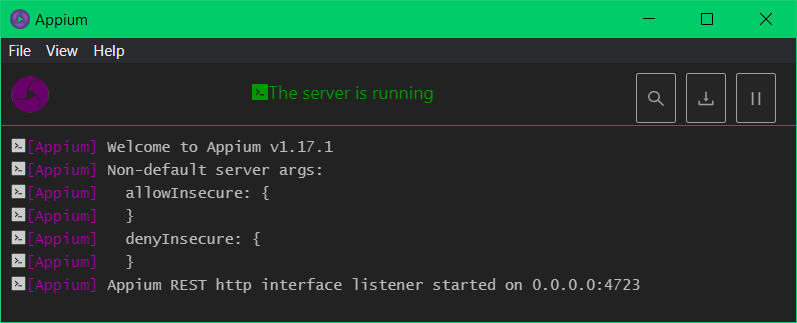
\includegraphics[scale=0.5]{appiumServer.png}
		\caption{Schermata del server Appium}\label{fig:appiumServer}
	\end{center}
\end{figure}

Di conseguenza Appium permette di utilizzare qualsiasi linguaggio o \gls{framework}\ap{[g]} che supporti l'invio di richieste HTTP inoltre, non è necessario compilare alcun codice o \gls{framework}\ap{[g]} specifico di Appium perché grazie al Mobile JSON Wire Protocol utilizza i framework per l'automazione dei \emph{test} come UIAutomator per\gls{Android}\ap{[g]} e XCTest per \gls{iOS}\ap{[g]}.


\section{Convezione}
Su suggerimento del tutor aziendale si è struttura la \emph{test-suite} da me implementata, nel seguente modo:\\
\begin{center}
	\begin{forest}
		for tree={font=\sffamily, grow'=0,
			folder indent=.9em, folder icons,
			edge=densely dotted}
		[e2e
		[test%, this folder size=20pt
		[feature%, this folder size=20pt
		[spec.feature, is file]
		]
		[step\_definition%, this folder size=20pt
		[spec.e2e-spec.ts, is file]
		]
		[pages%, this folder size=20pt
		[specs.po.ts, is file]
		]
		]
		]
	\end{forest}
\end{center}
\begin{itemize}
	\item \textbf{feature}: Contiene i file.feature dove vengono indicati gli scenari e gli \emph{step} dei \emph{test} scritti nell'linguaggio Gherkin. Ogni file.feature contiene test di scenari affini;
	\item \textbf{step\_definition}: Contiene i file.e2e-spec.ts dove vengono implementati gli \emph{step}, utilizzando i metodi dei file.po.ts. Esiste un file.e2e-spec.ts per ogni file.feature;
	\item \textbf{pages}: Contiene le cosiddette PageObject, le PageObject sono un design pattern che permettono di scrivere \emph{test} più puliti. Infatti, queste PageObject contengono metodi che vengono spesso riutilizzati da più \emph{test} e inoltre, estraggono gli elementi dalla vista. Adottando questo design pattern si ha il vantaggio che se il modello dell'applicazione cambia sarà sufficiente aggiornare solo la pageObject e inoltre si ha il vantaggio di non avere duplicazione del codice. Solitamente si creano più pageObject con metodi tra loro affini.
\end{itemize}
\section{Test eseguiti}
In comune accordo con il tutor aziendale, sono stati individuati i seguenti \emph{test} \gls{test e2e} che debbano testare l'intera applicazione \emph{mobile} quindi, non solo Azzurra ma anche le sezioni Questionario e Profilo. Inoltre sono stati testati anche alcuni aspetti della \emph{dashboard} di \gls{AWMS}\ap{[g]}. Per ogni \emph{test} viene assegnato un codice composto dalla lettera \textbf{T}, da una seconda lettera che può essere \textbf{M} nel caso in cui il \emph{test} sia per l'applicazione \emph{mobile}, oppure la lettera \textbf{D} se il \emph{test} è per la \emph{dashboard}. Infine il codice termina con un numero progressivo. Nella tabella sottostante per ogni \emph{test} viene riportato il suo codice, una descrizione e l'esito del \emph{test}.
\begin{table}[h]%
	\rowcolors{2}{grigetto}{white}
	\centering
	\begin{tabularx}{\textwidth}{c X c}
		\hline	
		\rowcolor{giallo}
		\intest{Codice} &  \intest{Descrizione} & \intest{Esito}\\	
		\hline			
		TM1 & Testare che l'utente possa inserire e-mail e password e cliccare il bottone invio per autenticarsi, nel caso i dati siano corretti l'utente deve essere renderizzato nella pagina Questionari. & Superato\\
		TM2 & Testare che l'utente possa inserire e-mail, password e cliccare il bottone invio per autenticarsi, nel caso i dati siano uno o tutti errati l'utente deve essere rimanere nella pagina di autenticazione. & Superato\\
		TM3 & Testare che nel caso in cui esista una versione più recente rispetto a quella in esecuzione, appaia all'apertura dell'applicazione un messaggio in primo piano che avvisi della nuova versione disponibile. & Superato\\
		TM4 & Testare che il messaggio in primo piano che avvisa della nuova versione disponibile, sia interagitile, cioè che si possa cliccare i suoi bottoni. & Superato\\
		TM5 & Testare che una volta che l'utente sia autenticato, se è il suo primo accesso, possa chiudere la finestra che contiene la guida per l'utilizzo dell'applicazione, la quale appare al primo accesso che si fa nell'applicazione. & Superato\\
		TM6 & Testare nella sezione Questionari, se la prima finestra del Questionario della salute (vedi la prima immagine della Figura~\ref{fig:queSlide}) abbia i vari bottoni dei sintomi tutti cliccabili. & Superato\\
			\end{tabularx} \hbox{}
	\caption{Tabella del tracciamento dei test \gls{test e2e}}
\end{table}%

\begin{table}[h]%
	\rowcolors{2}{grigetto}{white}
	\centering
	\begin{tabularx}{\textwidth}{c X c}
		\hline	
		\rowcolor{giallo}
		\intest{Codice} &  \intest{Descrizione} & \intest{Esito}\\	
		\hline	
		TM7 & Testare nella sezione Questionari, se la seconda finestra del Questionario della salute (vedi la seconda immagine della Figura~\ref{fig:queSlide}) abbia i vari bottoni sulla salute delle persone che vivono con te, siano tutti cliccabili. & Superato\\
		TM8 & Testare nella sezione Questionari, se la terza finestra del Questionario della salute (vedi la terza immagine della Figura~\ref{fig:queSlide}) abbia i vari bottoni dei posti in cui sei stato, siano tutti cliccabili. & Superato\\
		TM9 & Testare nella sezione Questionari, che venga visualizzato esito positivo(vedi prima immagine della Figur~\ref{fig:quefinal}) dalla compilazione del questionario se l'indice di contagiosità calcolato è basso. & Superato\\
		TM10 & Testare nella sezione Questionari, che venga visualizzato esito negativo(vedi seconda immagine della Figur~\ref{fig:quefinal}) dalla compilazione del questionario se l'indice di contagiosità calcolato è alto. & Superato\\
		TM11 & Testare nella sezione profilo che tutti i bottoni presenti siano cliccabili e che aprano la loro corrispondente finestra. & Superato\\
		TM12 & Testare nella sezione profilo, nella finestra Informazioni personali, se la ricerca degli indirizzi, per poter cambiare indirizzo di domicilio, produca risultati coerenti con quello che si sta cercando. & Superato\\
		TM13 & Testare nella sezione profilo, nella finestra Informazioni, si possa selezionare uno dei risultati della ricerca per il cambio dell'indirizzo di domicilio & Superato\\
		TM14 & Testare nella sezione profilo, nella finestra Informazioni, che tutti i bottoni siano cliccabili & Superato\\
		TM15 & Testare nella sezione profilo, nella finestra Informazioni, che le modifiche fatte a i dati una volta cliccato il bottone salva, rimangano salvate anche dopo la chiusura della finestra & Superato\\
		TM16 & Testare nella sezione profilo, Gestione password, si possa cambiare la password quindi che si possa inserire la password attuale, inserire una nuova password, la sua conferma e cliccare sul bottone salva. & Superato\\
		TM17 & Testare nella sezione profilo, che tutte le finestre aperte dopo il click sui bottoni, possano essere chiuse. & Superato\\
		TM18 & Testare nella sezione Azzurra, nella funzionalità "pianificazione" si possa visualizzare la pianificazione in uno specifico giorno. & Superato\\
		TM19 & Testare nella sezione Azzurra, nella funzionalità "Pianificazione" si possa visualizzare la pianificazione della settimana corrente. & Superato\\
		TM20 & Testare nella sezione Azzurra, nella funzionalità "Gestione assenze" si possa richiedere l'inserimento di una nuova assenza. & Superato\\
	\end{tabularx} \hbox{}
	\caption{Tabella del tracciamento dei test \gls{test e2e}}
\end{table}%

\begin{table}[h]%
	\rowcolors{2}{grigetto}{white}
	\centering
	\begin{tabularx}{\textwidth}{c X c}
		\hline	
		\rowcolor{giallo}
		\intest{Codice} &  \intest{Descrizione} & \intest{Esito}\\	
		\hline	
		TM21 & Testare nella sezione Azzurra, nella funzionalità "Gestione assenze" si possa visualizzare la lista delle assenze fatte. & Superato\\
		TM22 & Testare nella sezione Azzurra, nella funzionalità "Gestione assenze" si possa aprire il calendario dei giorni in cui si può prendere un permesso. & Superato\\
		TM23 & Testare nella sezione Azzurra, nella funzionalità "Prenotazione posto" che, si possa visualizzare le prenotazioni dei posti a sedere fatte. & Superato\\
		TM24 & Testare nella sezione Azzurra, nella funzionalità "Prenotazione posto" che, si possa una nuova prenotazione di un posto a sedere. & Superato\\
		TM25 & Testare nella sezione Azzurra, nella funzionalità "Prenotazione posto" che, si possa aprire lo scanner di \gls{QR code}\ap{[g]}. & Superato\\
		TM26 & Testare nella sezione Azzurra, che si possa aprire il menu delle shortcuts. & Superato\\
		TM27 & Testare che siano raggiungibili le sezioni Questionari, Azzurra, Profilo, dopo l'autenticazioni. & Superato \\
		TD28 & Testare nella sezione Task che all'inizio non ci sia nessun task selezionato. & Superato \\
		TD29 & Testare nella sezione Task che tutti i task siano selezionabili. & Superato \\
		TD30 & Testare nella sezione Task che una volta selezionato un task, appaia a lato un menu a tendina. & Superato \\
		TD31 & Testare nella sezione Task che la funzionalità di ricerca produca risultati coerenti con quanto si sta cercando. & Superato \\
		TD32 & Testare nella sezione Safety che tutti i bottoni siano cliccabili e nel caso in cui aprano delle nuove finestre, queste possano essere chiuse. & Superato \\
		TD31 & Testare nella sezione Safety che la funzionalità di ricerca produca risultati coerenti con quanto si sta cercando. & Superato \\
	\end{tabularx} \hbox{}
	\caption{Tabella del tracciamento dei test \gls{test e2e}}
\end{table}%
